\documentclass{article}

\usepackage[utf8]{inputenc}
\usepackage[backend=biber, style=numeric]{biblatex}
\usepackage[dutch]{babel}
\usepackage{fancyhdr}
\usepackage{graphicx}
\usepackage{booktabs}
\usepackage{float}
\usepackage{wrapfig}
\usepackage{listings}
\usepackage{color}

\definecolor{codegreen}{rgb}{0,0.6,0}
\definecolor{codegray}{rgb}{0.5,0.5,0.5}
\definecolor{codepurple}{rgb}{0.58,0,0.82}
\definecolor{backcolour}{rgb}{0.95,0.95,0.92}

\lstdefinestyle{codestyle}{
    backgroundcolor=\color{backcolour},   
    commentstyle=\color{codegreen},
    keywordstyle=\color{magenta},
    numberstyle=\tiny\color{codegray},
    stringstyle=\color{codepurple},
    basicstyle=\footnotesize,
    breakatwhitespace=false,         
    breaklines=true,                 
    captionpos=b,                    
    keepspaces=true,                 
    numbers=left,                    
    numbersep=5pt,                  
    showspaces=false,                
    showstringspaces=false,
    showtabs=false,                  
    tabsize=2
}
 
\lstset{style=codestyle}


\pagestyle{fancy}
\fancyhf{}
\rhead{ Scaling }
\lhead{Meetrapport, Snelheid}
\rfoot{Pagina \thepage }

\begin{document}
\author{Dimitry Volker}
\makeatletter
    \begin{titlepage}
        \begin{center}
            {\huge \bfseries  \@title }\\[2ex] 
            {\LARGE Meetrapport, Snelheid - Scaling}\\[10ex]
            
            {\large \@author - 1661152}\\
            {\large Jasper van Hulst - 1660498}\\[5ex]
            {\large \@date}
            
            \vskip4em%
        \end{center}
    \end{titlepage}
\makeatother
\thispagestyle{empty}

\clearpage

\renewcommand{\contentsname}{Inhoudsopgave}
\tableofcontents

\clearpage

\section{Doel}
Het schalen van een afbeelding is op diverse manieren voor elkaar te krijgen. Er bestaan 3 algoritmes die veel op elkaar lijken "Nearest-neighbour Interpolation", "Bilinear Interpolation" en "Bicubic Interpolation". Wanneer er een situatie voorkomt waar je bijvoorbeeld heel veel afbeeldingen moet scalen, dan is het belangrijk om te weten wat de snelste is, ongeacht de kwaliteit. Daarom stellen wij de volgende vraag:

\begin{center}
    "Welk algoritme is het snelst voor scaling?".   
\end{center}

\section{Hypothese}

Het lijkt ons dat de Nearest-neighbour op alle experimenten het snelste zal presteren. Er zijn bijna geen calculaties en er word alleen gekeken naar de "dichtstbijzijnde" pixel. 

\clearpage

\section{Onderzoeksmethode}
Om een goed beeld te krijgen naar de snelheid van de drie algoritmes worden de experimenten tien keer uitgevoerd per schalingsfactor. Hier kijken wij naar het verkleinen en vergroten van een afbeelding vanaf de orginele grote. 

\begin{figure}[H]
    \centering
    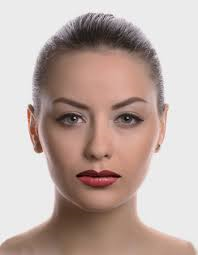
\includegraphics{assets/female-3.png}
    \caption{Orginele afbeelding}
    \label{fig:my_label}
\end{figure}

\begin{table*}[h] \centering
\begin{tabular}{l}
    0.5x \\
    0.75x \\
    1.25x \\
    1.50x \\
\end{tabular}
\caption{Geteste schalingsfactoren}
\end{table*}

\newpage
\subsection{Code}

\begin{lstlisting}[language=C++, caption=Code voor timen]
#include <time.h>
clock_t start, finish;
...

for (int i = 0; i < 10; i++) {
    result = ImageFactory::newIntensityImage(WIDTH, HEIGHT);
    start = clock();
    
    //scaling here //
    
    finish = clock();
    std::cout << "Time for x (seconds):"
    << ((double)(finish - start)) / CLOCKS_PER_SEC;
    delete result;
}
\end{lstlisting}

\clearpage
\section{Resultaten}
Zoals aangegeven in hoofdstuk 3, word de afbeelding geschaald met diverse schalingsfactoren. Om een goed resultaat te krijgen word elke test 10 keer uitgevoerd. 

\subsection{Schalingsfactor 0.5}

\begin{table}[H]
    \centering
    \begin{tabular}{ccc}
        \toprule
            Nearest-neighbor interpolation & \multicolumn{1}{l}{Bilinear Interpolation} &\multicolumn{1}{l}{Bicubic Interpolation} \\
        \midrule
            0,005s & 0,009s & 0,026s  \\
            0,003s & 0,006s & 0,024s  \\
            0,004s & 0,007s & 0,024s  \\
            0,003s & 0,006s & 0,023s  \\
            0,003s & 0,007s & 0,024s  \\
            0,003s & 0,007s & 0,024s  \\
            0,003s & 0,007s & 0,023s  \\
            0,004s & 0,006s & 0,023s  \\
            0,003s & 0,006s & 0,024s  \\
            0,003s & 0,007s & 0,027s  \\
    \end{tabular}
    \caption{Resultaten schalen met factor 0.5}
\end{table}

\begin{figure}[H]
    \centering
    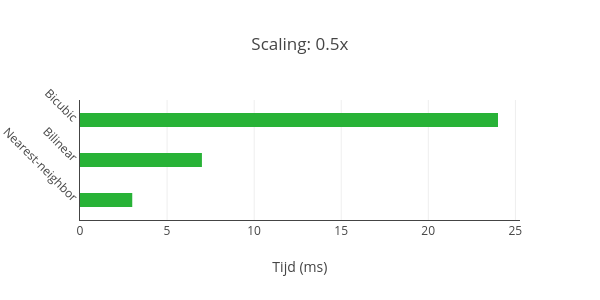
\includegraphics[width=12cm]{graphs/Scaling_05.png}
    \caption{Gemiddelde lengte van schalen met factor 0.5}
    \label{fig:my_label}
\end{figure}

\subsection{Schalingsfactor 0.75}

\begin{table}[H]
    \centering
    \begin{tabular}{ccc}
        \toprule
            Nearest-neighbor interpolation & \multicolumn{1}{l}{Bilinear Interpolation} &\multicolumn{1}{l}{Bicubic Interpolation} \\
        \midrule
            0,008 & 0,015 & 0,055 \\
            0,007 & 0,015 & 0,059 \\
            0,007 & 0,015 & 0,056 \\
            0,007 & 0,015 & 0,053 \\
            0,007 & 0,015 & 0,051 \\
            0,009 & 0,016 & 0,052 \\
            0,007 & 0,021 & 0,058 \\
            0,007 & 0,015 & 0,055 \\
            0,007 & 0,015 & 0,052 \\
            0,007 & 0,017 & 0,052 \\
    \end{tabular}
    \caption{Resultaten schalen met schaalfactor 0.75}
\end{table}

\begin{figure}[H]
    \centering
    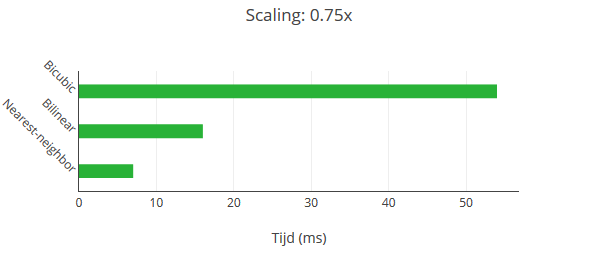
\includegraphics[width=12cm]{graphs/Scaling_075.PNG}
    \caption{Gemiddelde lengte van schaling met factor 0.75}
    \label{fig:my_label}
\end{figure}

\subsection{Schalingsfactor 1.25}

\begin{table}[H]
    \centering
    \begin{tabular}{ccc}
        \toprule
            Nearest-neighbor interpolation & \multicolumn{1}{l}{Bilinear Interpolation} &\multicolumn{1}{l}{Bicubic Interpolation} \\
        \midrule
            0,020 & 0,048 & 0,162 \\
            0,020 & 0,047 & 0,146 \\
            0,020 & 0,052 & 0,152 \\
            0,022 & 0,043 & 0,146 \\
            0,023 & 0,044 & 0,145 \\
            0,019 & 0,041 & 0,145 \\
            0,019 & 0,042 & 0,145 \\
            0,019 & 0,050 & 0,144 \\
            0,018 & 0,044 & 0,146 \\
            0,019 & 0,041 & 0,145 \\
            0,020 & 0,045 & 0,148 \\
    \end{tabular}
    \caption{Resultaten schalen met schaalfactor 1.25}
\end{table}

\begin{figure}[H]
    \centering
    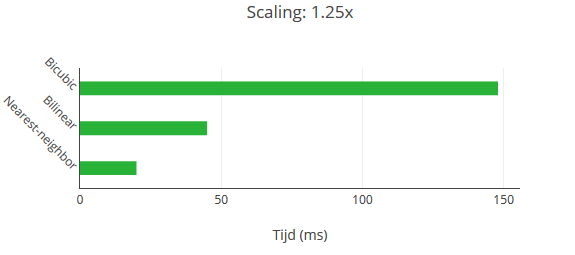
\includegraphics[width=12cm]{graphs/Scaling_125.PNG}
    \caption{Gemiddelde lengte van schaling met factor 1.25}
    \label{fig:my_label}
\end{figure}

\subsection{Schalingsfactor 1.5}

\begin{table}[H]
    \centering
    \begin{tabular}{ccc}
        \toprule
            Nearest-neighbor interpolation & \multicolumn{1}{l}{Bilinear Interpolation} &\multicolumn{1}{l}{Bicubic Interpolation} \\
        \midrule
            0,027 & 0,059 & 0,222 \\
            0,034 & 0,062 & 0,220 \\
            0,034 & 0,063 & 0,216 \\
            0,033 & 0,070 & 0,210 \\
            0,036 & 0,061 & 0,211 \\
            0,033 & 0,062 & 0,210 \\
            0,028 & 0,061 & 0,208 \\
            0,029 & 0,062 & 0,206 \\
            0,028 & 0,063 & 0,206 \\
            0,028 & 0,060 & 0,210 \\
    \end{tabular}
        \caption{Resultaten schalen met schaalfactor 1.50}
\end{table}

\begin{figure}[H]
    \centering
    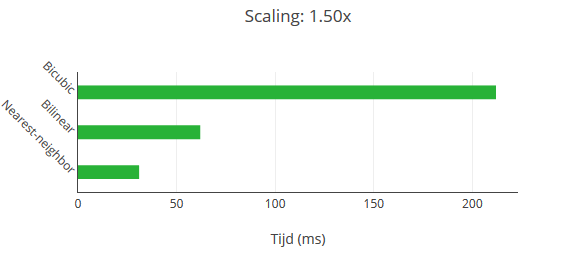
\includegraphics[width=12cm]{graphs/Scaling_150.PNG}
    \caption{Gemiddelde lengte van schaling met factor 1.50}
    \label{fig:my_label}
\end{figure}

\section{Conclusie}
Uit de resultaten kunnen we concluderen dan, ongeacht vergroten of verkleinen, de "Nearest-Neighbour Interpolatie" het snelste algoritme van de 3 is. 


\end{document}